%----------------------------------------------------------------------------
\chapter{Mérési eredmények}
%----------------------------------------------------------------------------

Ebben a fejezetben a tesztek eredményének elemzéséről és a leszűrhető konklúziókról lesz szó. Az elkészült program és a Train Benchmark többi tesztjének futtatása sok órás művelet. A kigenerált modellek mérete

\section{\emph{Inject}}
\pagebreak
\begin{figure}[H]
	\centering
	\vspace*{-2cm}
	\makebox[\linewidth]{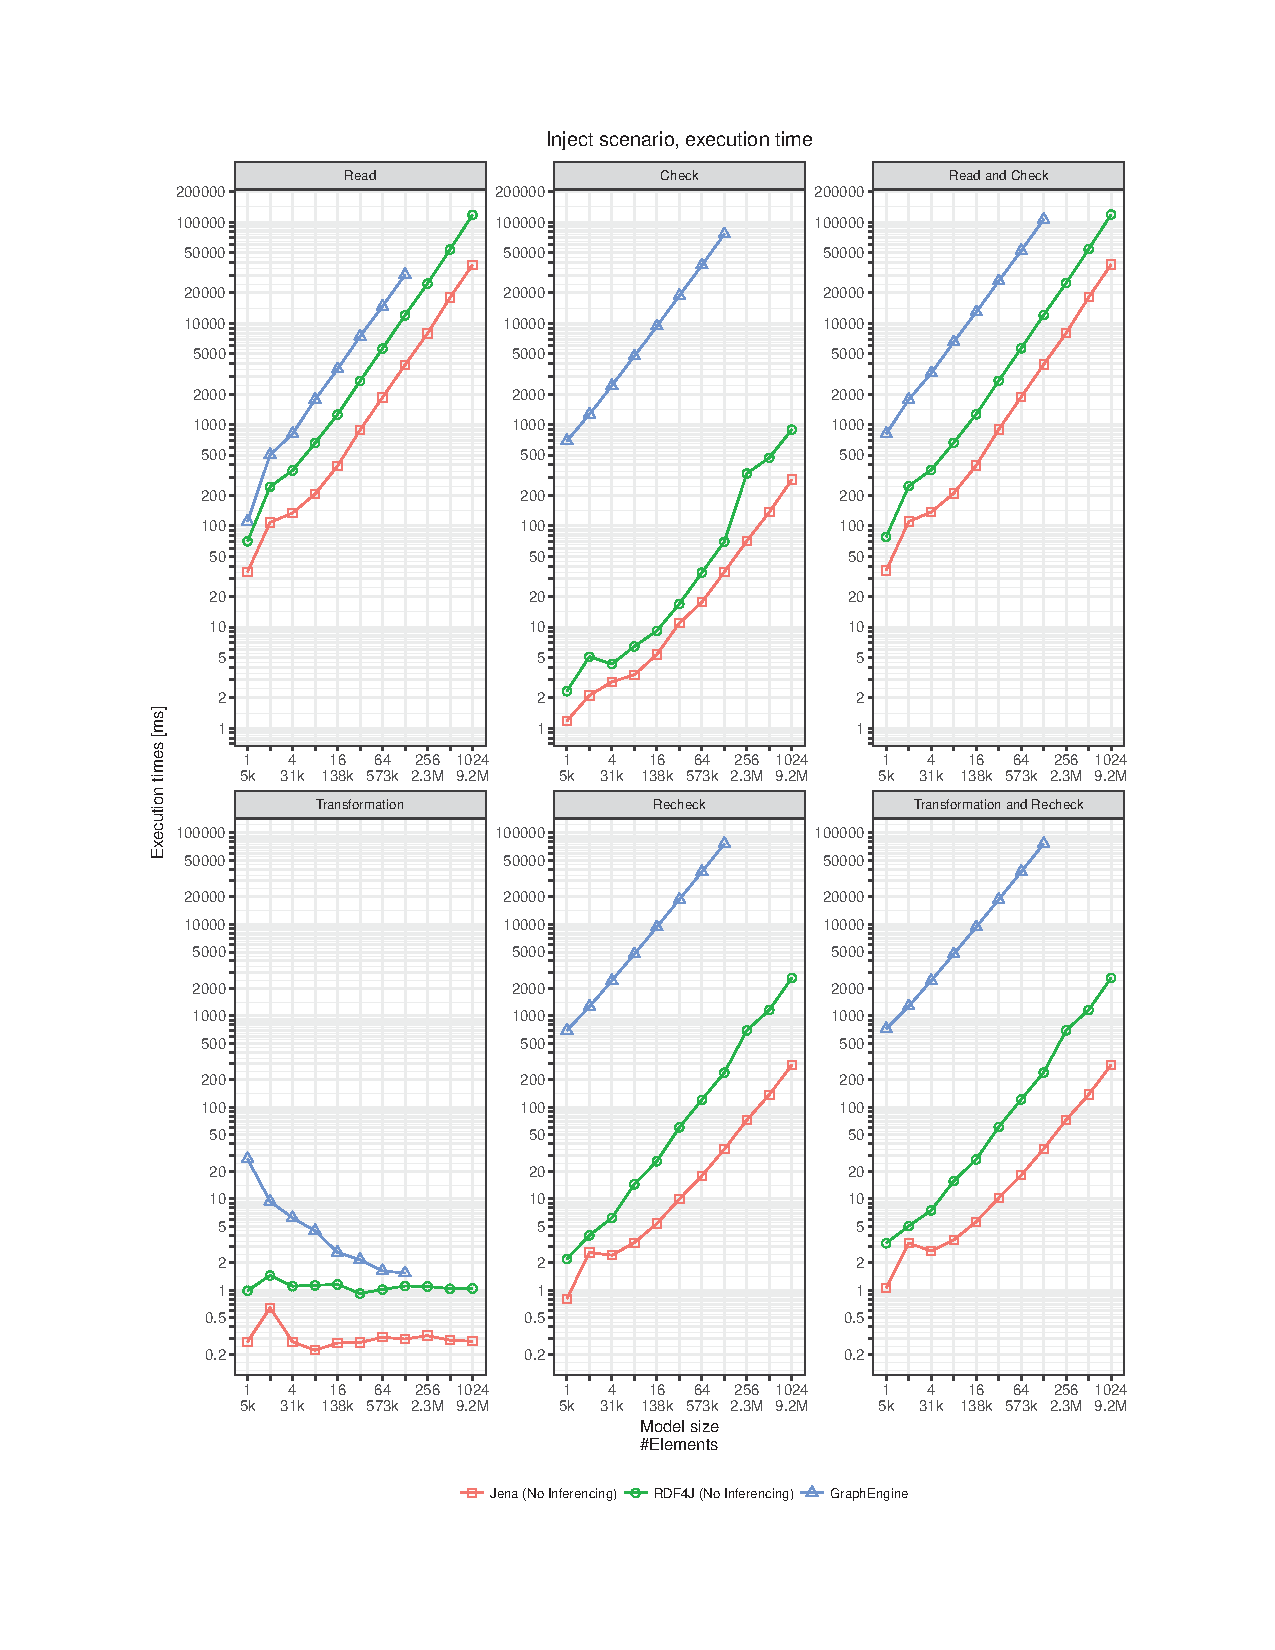
\includegraphics[width=1.3\linewidth]{figures/times-Inject.pdf}}
	\label{fig:InjectResult}
	\caption{Az \emph{Inject} szakasz futási idejeinek eredménye.}
\end{figure}


%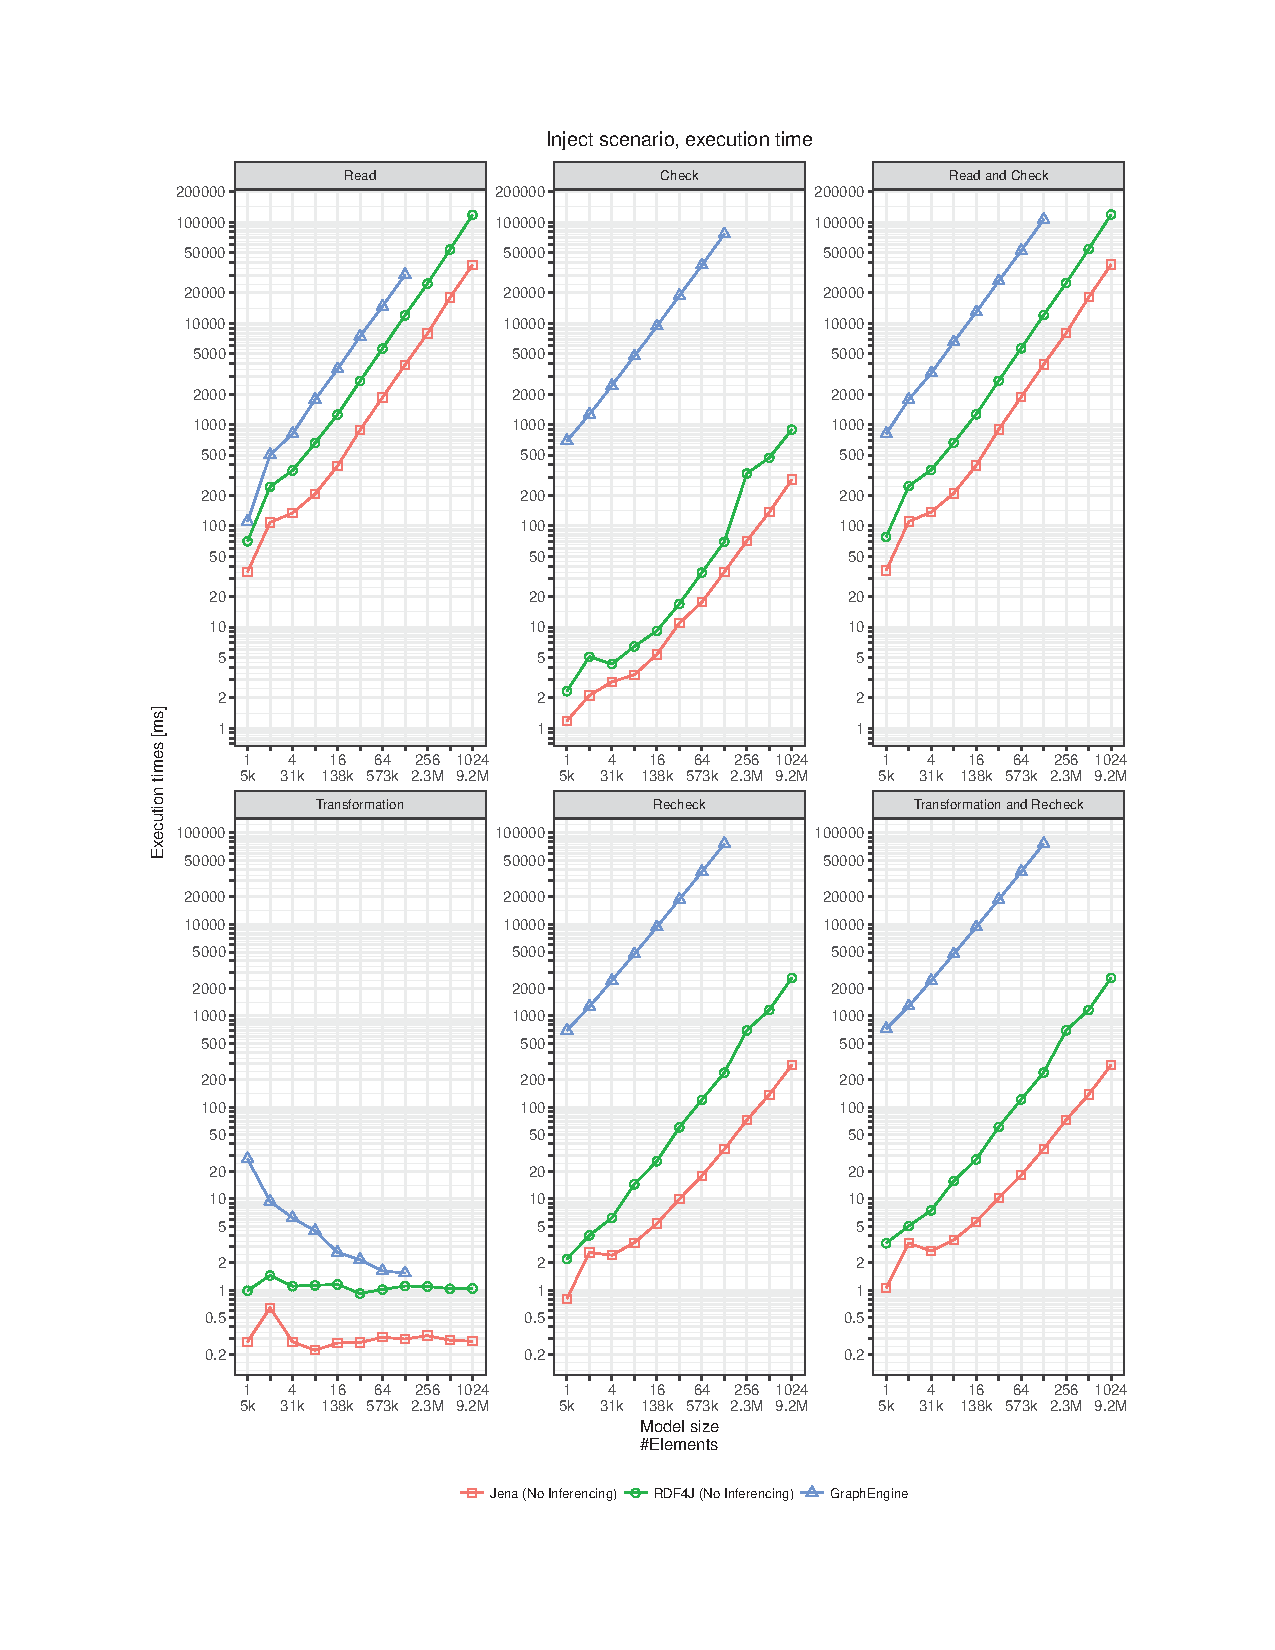
\includepdf[pagecommand={}]{figures/times-Inject.pdf}\label{fig:injectResult}

\section{\emph{Repair}}

\pagebreak
\begin{figure}[H]
	\centering
	\vspace*{-2cm}
	\makebox[\linewidth]{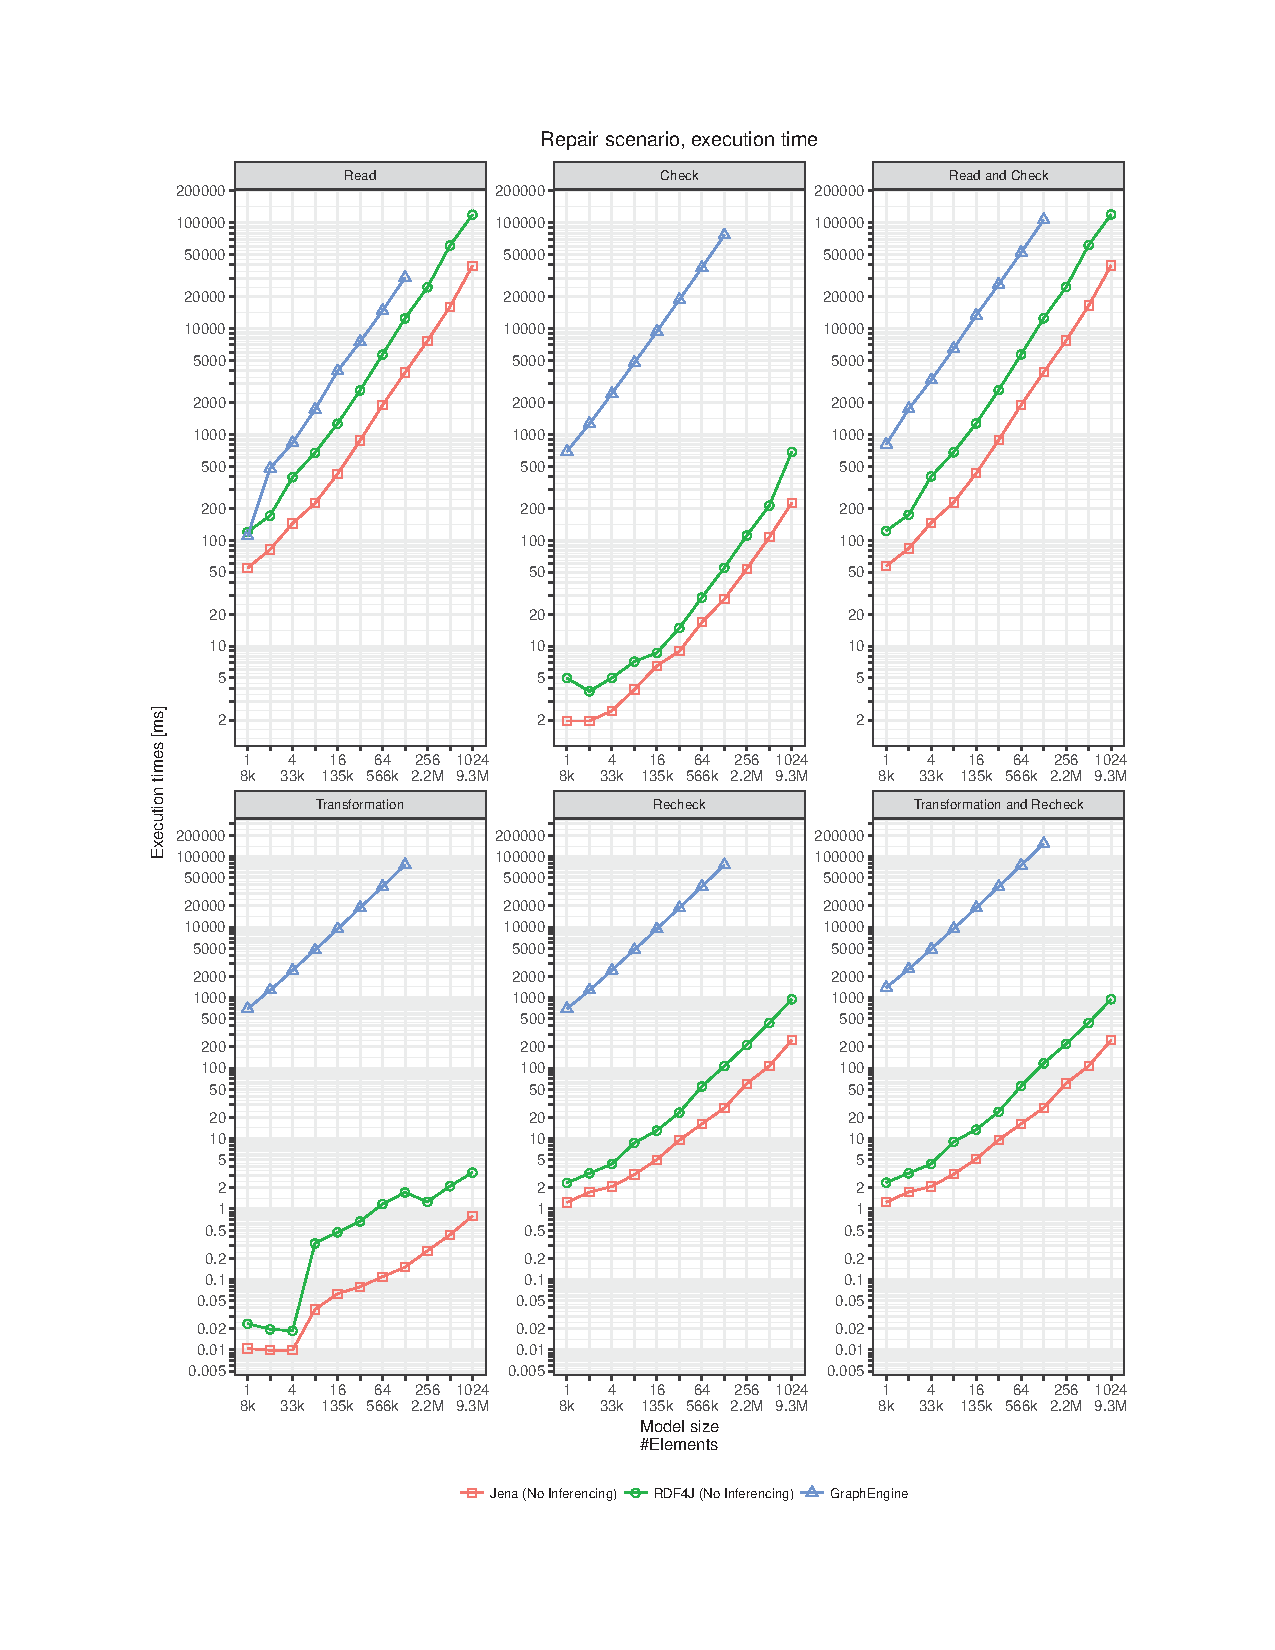
\includegraphics[width=1.3\linewidth]{figures/times-Repair.pdf}}
	\label{fig:RepairResult}
	\caption{A \emph{Repair} szakasz futási idejeinek eredménye.}
\end{figure}

%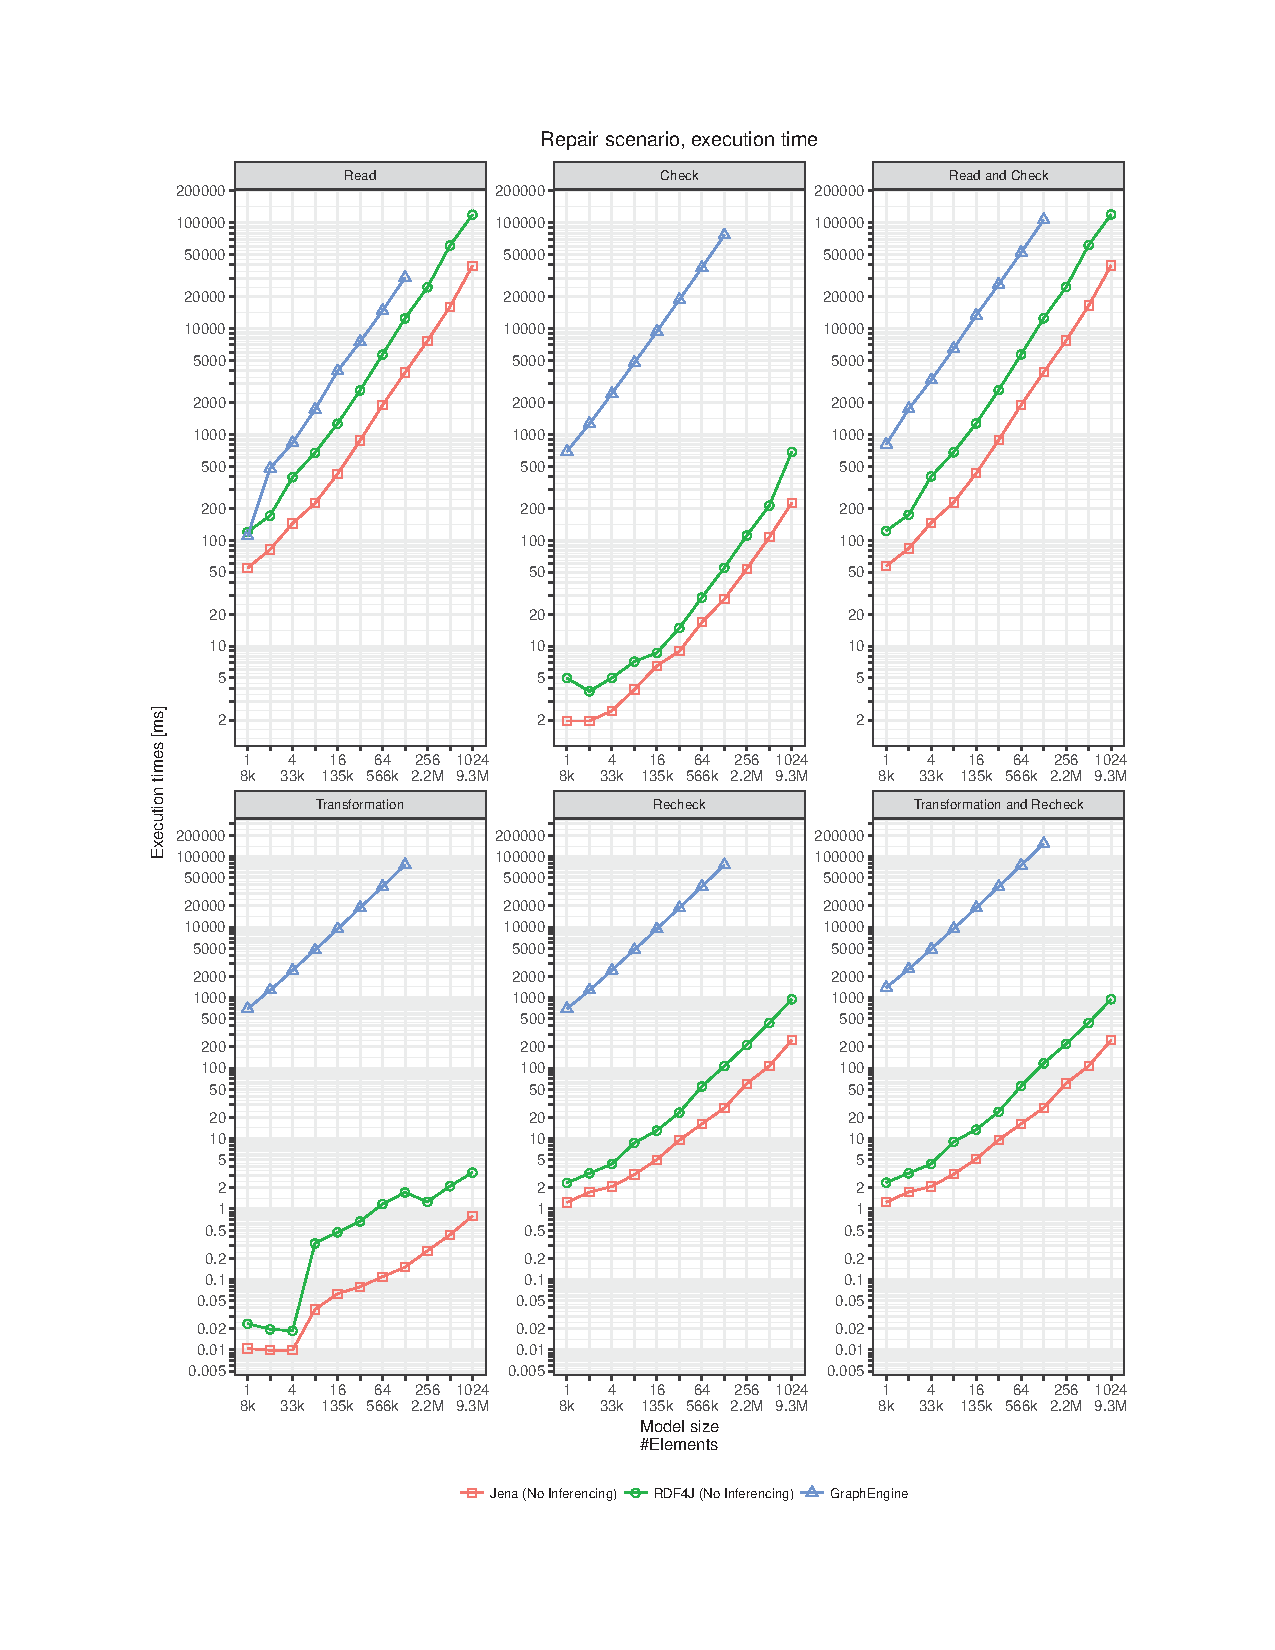
\includepdf[pagecommand={}]{figures/times-Repair.pdf}